%\modeCorrection

\renewcommand{\thesubsection}{\textcolor{red}{\Roman{section}.\arabic{subsection}}}
\renewcommand{\thesubsubsection}{\textcolor{red}{\Roman{section}.\arabic{subsection}.\alph{subsubsection}}}

\setcounter{section}{0}
\enTeteChap{6}{De l'espèce chimique à l'entité.}

\begin{mdframed}[style=titr, leftmargin=60pt, rightmargin=60pt, innertopmargin=7pt, innerbottommargin=7pt, innerrightmargin=8pt, innerleftmargin=8pt]

\begin{center}
\large{\textbf{Chapitre 6 : De l'espèce chimique à l'entité.}}
\end{center}
\end{mdframed}


\begin{tcolorbox}[colback=blue!5!white,colframe=blue!75!black,title=Mots clés du chapitre :]
Echelle macroscopique, échelle microscopique, espèce chimique, entité chimique, composé ionique, électroneutralité, quantité de matière
\end{tcolorbox}


\section{Constitution de la matière}
\subsection{\`{A} l'échelle microscopique}
On dénombre trois entités chimiques qui structure la matière à l'échelle microscopique :
\begin{center}
    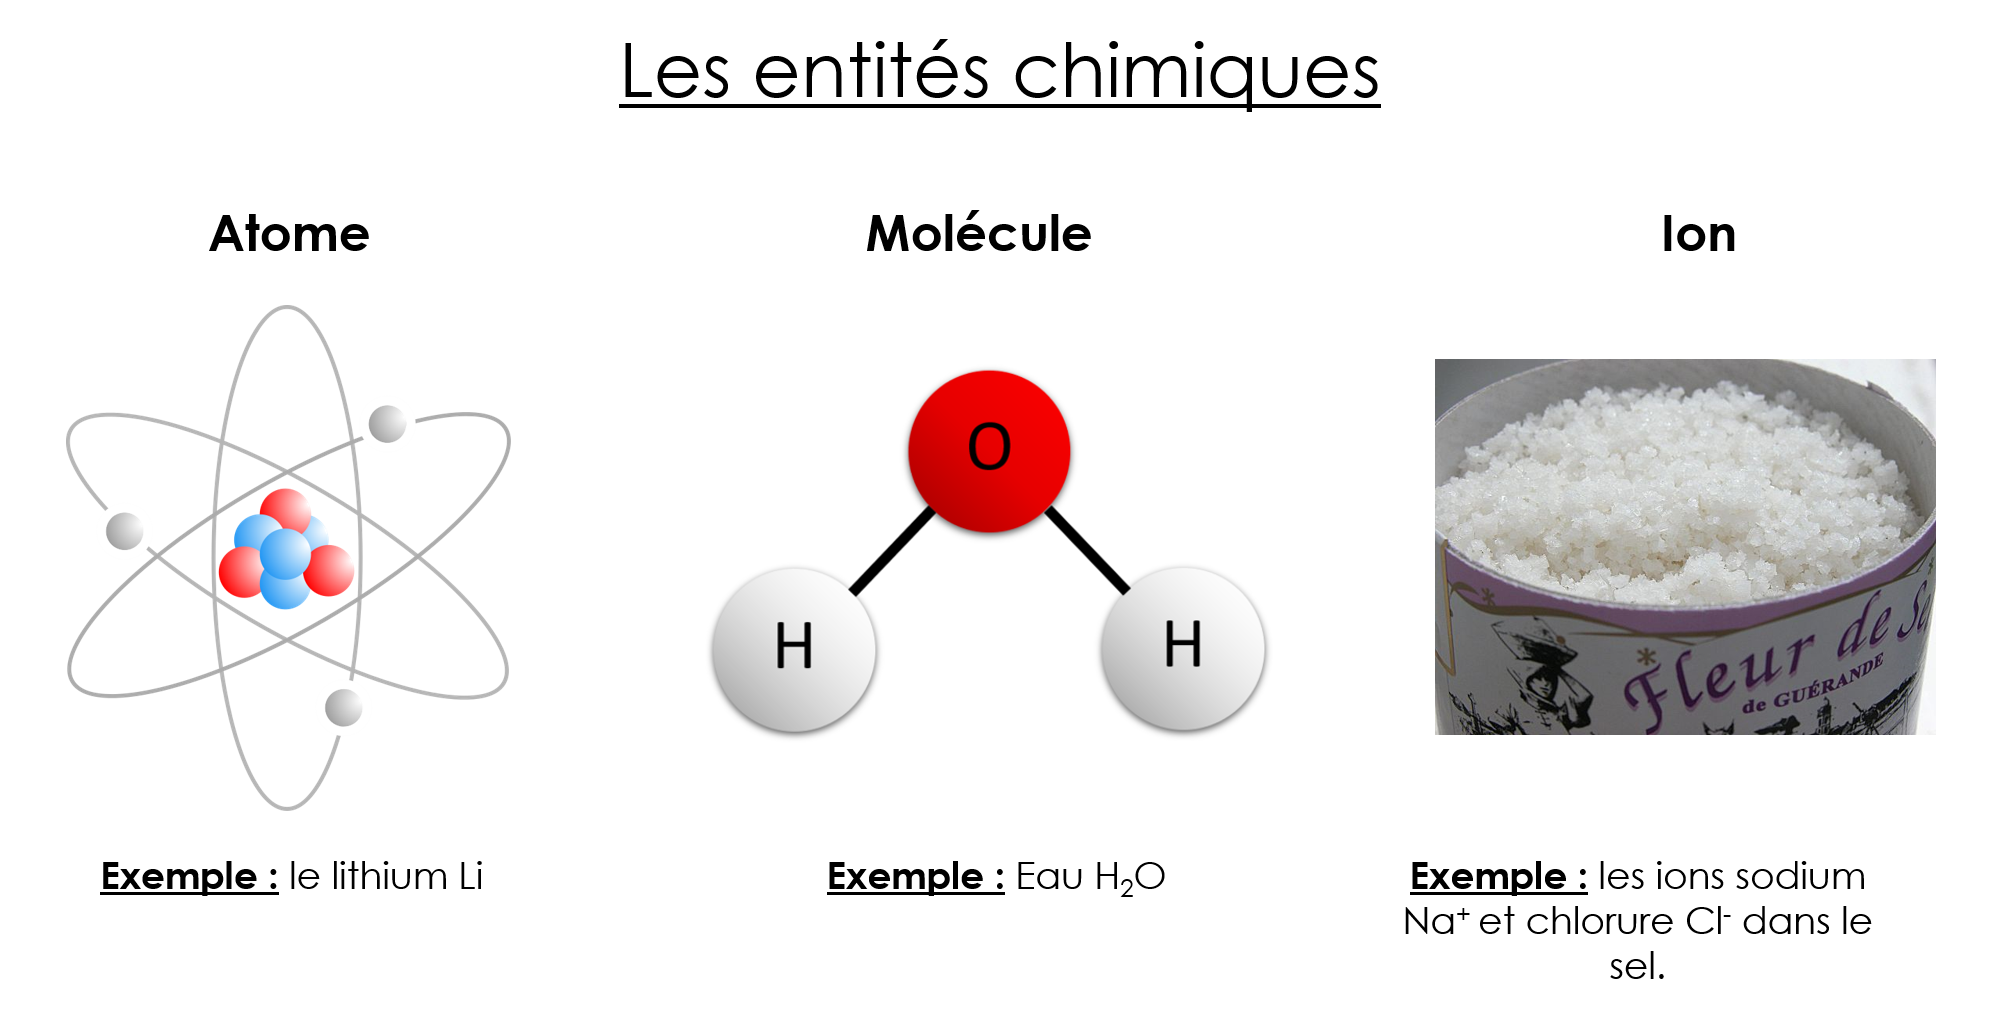
\includegraphics[scale=0.5]{Images/Entites_chimiques.png}
\end{center}

\begin{tcolorbox}[colback=green!5!white,colframe=green!75!black,title=\textbf{Définitions :}]
\begin{itemize}[label=\textbullet, font=\large]
    \item Un atome est la plus petite entité chimique électriquement neutre qui identifie un élément chimique du tableau périodique ;
    \item Une molécule est une entité chimique électriquement neutre constituée d'au moins deux atomes ;
    \item Un ion est une entité chimique porteuse d'une charge électrique. 
\end{itemize}

\end{tcolorbox}

\subsection{\`{A} l'échelle macroscopique : retour sur l'espèce chimique}
Dans le Chapitre 1 : Corps purs et mélanges au quotidien, nous avons définis une espèce chimique comme un ensemble (un très très grand nombre !) d'entités chimiques avec des propriétés physiques et chimiques. Une espèce chimique est intrinsinquèment liée à l'entité chimique qui la constitue et des intéractions que ces entités peuvent avoir entre elles à l'échelle microscopique.

\begin{center}
    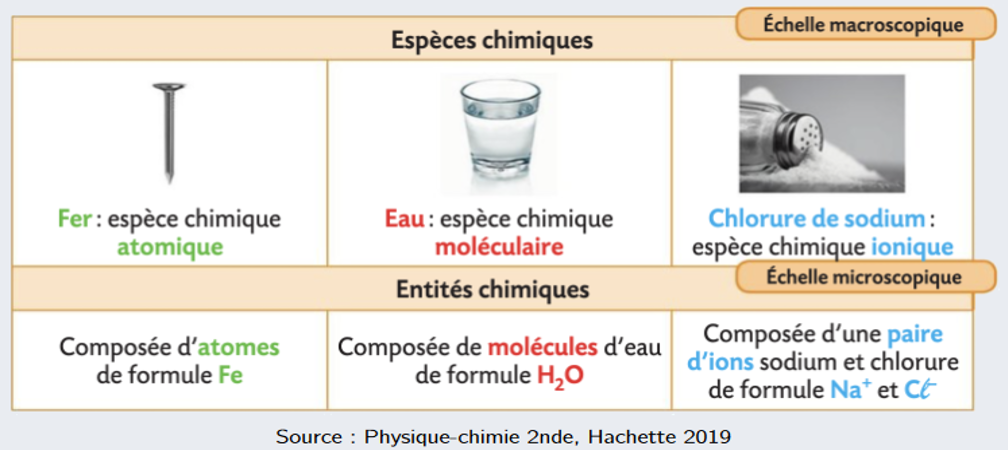
\includegraphics[scale=1]{Images/MicroVSMacro.png}
\end{center}
\subsection{Cas particulier des composés ioniques}
\begin{Large}
    \ding{43}
\end{Large}
Voir TP 12 : \'{E}tude des composés ioniques.
\begin{center}
    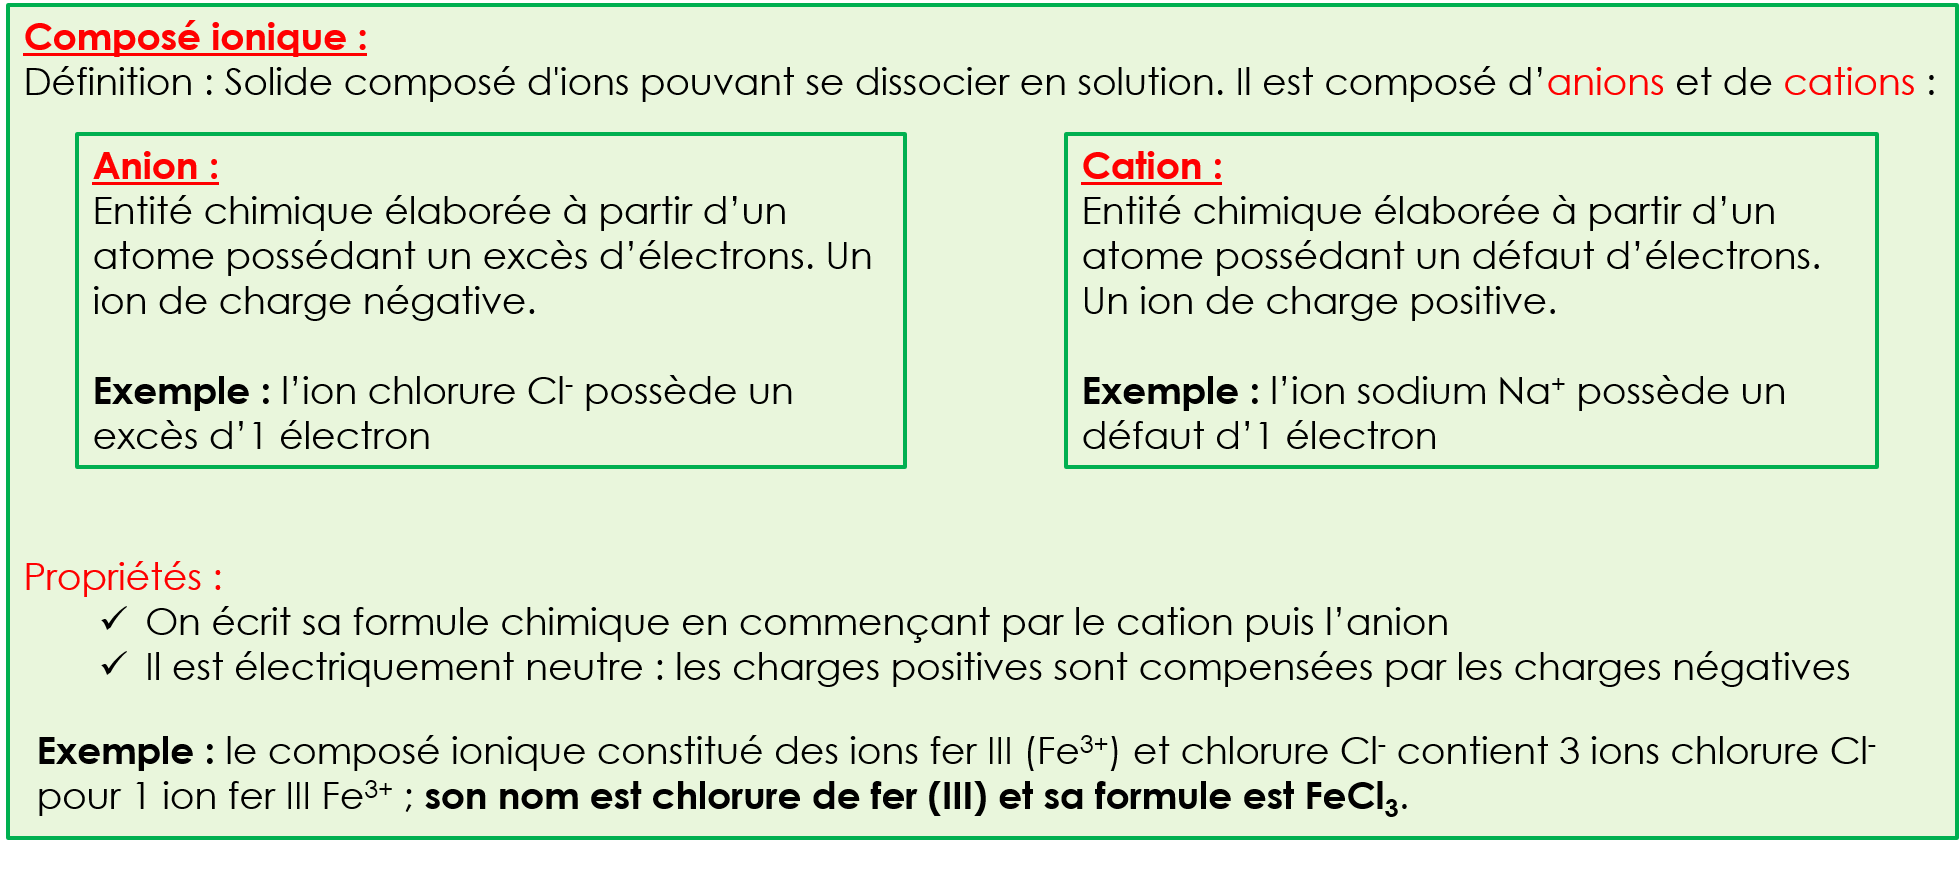
\includegraphics[scale=0.57]{Images/Solide_ionique.png}
\end{center}

\begin{Large}
    \ding{45}
\end{Large}\textbf{Partie I de la feuille d'exercices. Exercice : QCM, 6, 12, 15, 16}
\newpage
\section{La quantité de matière}
\begin{Large}
    \ding{43}
\end{Large}
Voir Activité : Dénombrer les entités dans le basilic.
\subsection{Détermination de la masse d'une entité}
\begin{tcolorbox}[colback=red!5!white,colframe=red!75!black,title=\textbf{Règle sur les molécules et les ions polyatomiques : }]
\begin{itemize}[label=\textbullet, font=\large]
    \item La masse des molécules se calcule en faisant la somme des masses de chacun des atomes la constituant. Exemple pour le glucose de formule chimique \chemform{C_6H12O6} : 
        \begin{equation*}
            m(\text{\chemform{C_6H_{12}O_6}}) = 6\times m(C) + 12\times m(H) + 6\times m(O)
        \end{equation*}
    \item C'est la même règle pour déterminer la masse d'un ion polyatomique. Exemple pour l'ion sulfate de formule chimique \chemform{SO_4}$^{-2}$ :
        \begin{equation*}
            m(\text{\chemform{SO_4}$^{-2}$}) = 1\times m(S) + 4\times{O}
        \end{equation*}
\end{itemize}

\end{tcolorbox}

\subsection{Dénombrer les entités : la mole}
On peut calculer le nombre d'entités chimiques présents dans un échantillon de masse $m_{ech}$ à partir de la masse des atomes présents dans cette espèce : 
\begin{itemize}[label=\textbullet, font=\large]
    \item 1 entité $\rightarrow$ $m_{\text{entité}}$
    \item N entités dans l'espèce chimique $\rightarrow$ $m_{ech}$
    \item d'où N$=\frac{m_{ech}}{m_{\text{entité}}}$
\end{itemize}
En chimie, travailler avec un nombre d'entités chimiques est compliqué puisque le calcul donne N très très grand ! Plutôt que de compter en entités, on décide de les rassembler par paquet appelé : \textcolor{red}{mole}.
\begin{tcolorbox}[colback=green!5!white,colframe=green!75!black,title=\textbf{La mole :}]
Une \textcolor{red}{mole} d'une espèce chimique contient un extrêmement grand d'entités chimiques la constituant. En appelant $N$ le nombre d'entités chimiques et $n$ le nombre de moles d'une espèce chimique, il existe : 
\begin{empheq}[box=\fbox]{equation*}
    N = n\times\mathrm{N_A}\text{ ou alors } n=\frac{N}{\mathrm{N_A}}
\end{empheq}
entités chimiques dans $n$ moles d'espèce chimique. $\mathrm{N_A}$ est appelé \textcolor{red}{constante d'Avogadro} et vaut : 
\begin{empheq}[box=\fbox]{equation*}
    \mathrm{N_A} = 6,022\times10^{23}\text{mol$^{-1}$}
\end{empheq}
Elle représente le nombre d'entités chimiques par mole de composé. Elle fait donc le lien entre l'échelle microscopique (l'entité) et l'échelle macroscopique (l'espèce chimique).
\end{tcolorbox}

\begin{Large}
    \ding{45}
\end{Large}\textbf{Partie II de la feuille d'exercices : Exercices 8, 10, 12, 16, 17, 26}